\chapter{Pilastro}

In questo capitolo si progetterà e verificherà il pilastro P27 secondo l'azione assiale precedentemente riportata in figura \ref{fig:AndamentoP27} di pagina \pageref{fig:AndamentoP27}, di cui si riporta qui sotto l'azione massima alla base del pilastro:
\begin{equation}
    N_{Ed} = \SI{1416.00}{\kilo\newton} \quad N_{EQP} = \SI{829.35}{\kilo\newton}
\end{equation}
\section{Progetto pilastro alla base e verifica compressione}
Per determinare l'area minima di calcestruzzo e di acciaio le \norma{NTC18} propongono le seguenti formule al \normaref{4.1.6.1.2}:
\begin{align}
    A_{s,min} &= 0.10\,\frac{N_{Ed}}{f_{yd}}  > 0.003 \, A_c \\
    A_c &= 0.90\,\frac{N_{Ed}}{f_{cd}}
\end{align}
i quali diventano rispettivamente $\SI{361.87}{\milli\metre\squared}$ e $\SI{299.93}{\milli\metre}$.

Scegliendo 2+2Ø12 = $\SI{452.16}{\milli\metre\squared}$ e  $\SI{300}{\milli\metre}$ come base del pilastro, la verifica risulta:
\begin{equation}
    N_{Rd} = 0.8 A_c f_{fcd} + A_s f_{yd} = \SI{1197}{\kilo\newton} < N_{Ed} = \SI{1416.00}{\kilo\newton} \quad \notchecked
\end{equation}

Viene pertanto aumentata la base a $\SI{350}{\milli\metre}$, che però ciò implica il dover disporre di una barra aggiuntiva, in quanto si avrebbe la distanza tra le barre di spigolo maggiore di $\SI{300}{\milli\metre}$.
Viene inoltre aumentato il diametro a 14, perciò si avranno 3+3Ø14 = $\SI{923}{\milli\metre\squared}$.
Occorre inoltre dover aumentare l'azione sollecitante, perché calcolata con un predimensionamento della precedente base. 
Vengono aggiunti quindi \SI{9.75}{\kilo\newton} al $G_1$, corrispondenti al peso proprio aggiuntivo, per l'intera altezza dell'edificio.
L'azione SLU diviene quindi $N_{Ed} = \SI{1425.75}{\kilo\newton}$. 
La verifica a compressione risulta soddisfatta:

\begin{equation}
    N_{Rd} = 0.8 A_c f_{fcd} + A_s f_{yd} = \SI{1749.77}{\kilo\newton} > N_{Ed} = \SI{1425.75}{\kilo\newton} \quad \checked \quad .
\end{equation}
Il quantitativo massimo di armatura è inoltre soddisfatto:
\begin{equation}
    A_s =
      \SI{923}{\milli\metre\squared} 
    \begin{cases}
      < 0.04 \, A_c = 0.04 \, b \, h = \SI{9000}{\milli\metre\squared} \\
      > 0.003 \, A_c = 0.003 \, b \, h = \SI{367.50}{\milli\metre\squared}
    \end{cases}
    \quad \checked
  \end{equation}

Per quanto riguarda l'armatura trasversale a taglio si deve avere:
\begin{align}
    s_{st,min} &= \min\left( 12\varnothing_{long.} \, ; \, \SI{250}{\milli\metre} \right)= \SI{168}{\milli\metre}\\
    \varnothing_{st, min} &= \max\left( 0.25\varnothing_{long.} \, ; \, \SI{6}{\milli\metre} \right)= \SI{6}{\milli\metre}
\end{align}
Da cui si scelgono staffe a due bracci Ø8/\SI{150}{\milli\metre}

\section{Verifica presso-flessione}
Sebbene il pilastro sia sottoposto a puro sforzo assiale, la normativa richiede di considerare un minimo quantito di eccentricità calcolabile come
\[
    e_0 = \max \left(\frac{l_0}{200};  \SI{20}{\milli\metre} \right)  = \max \left(\frac{3500}{200};  20 \right)\si{\milli\metre} = \SI{20}{\milli\metre}
\]
la quale genera un momento flettente pari a 
\begin{equation}
    M_{Ed} = N_{Ed}\cdot e_0  = \SI{1425.75}{\kilo\newton} \cdot (\SI{20}{\milli\metre} = \SI{28.52}{\kilo\newton\metre}
\end{equation}

Per verificarne la resistenza a presso-flessione si fa uso del diagramma M-N che permette di rappresentare la resistenza della sezione  per tutti i valori possibili di azione assiale.
Tale diagramma è riportato in figura \ref{fig:MN_diagram_primo_ordine}, dimostrando che la verifica è soddisfatta.
\begin{figure}[H]
    \centering
    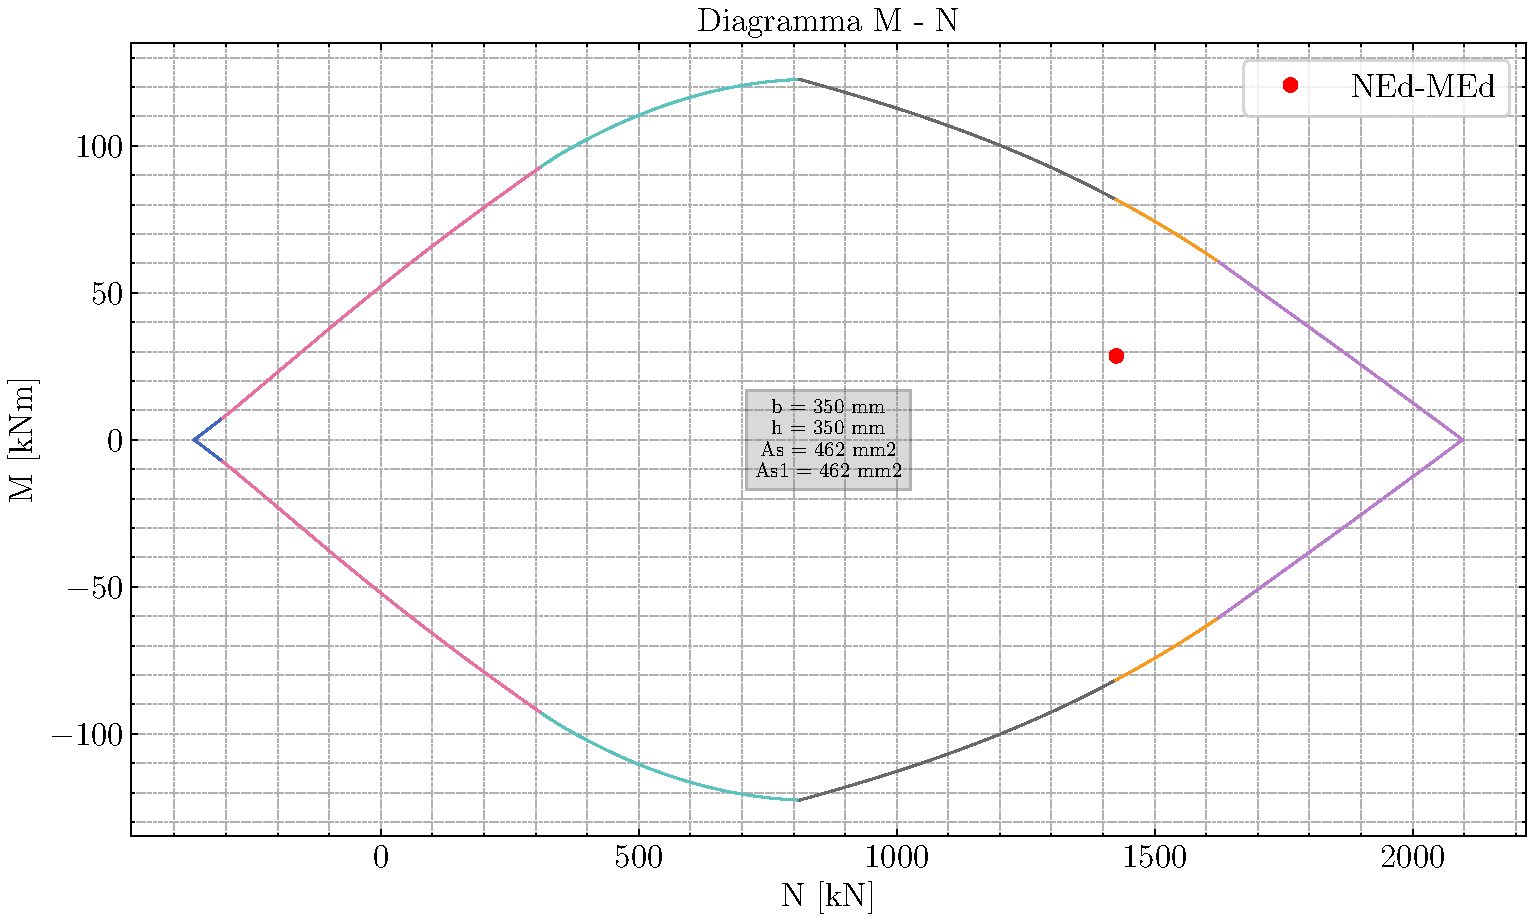
\includegraphics[width=\textwidth]{IMG/M_N_diagram_pilastro_primo_ordine.pdf}
    \caption{Diagramma MN presso-flessione}
    \label{fig:MN_diagram_primo_ordine}
\end{figure}


\section{Verifica di stabilità}
Occorre innanzitutto controllare se la snellezza reale del pilastro superi o meno quella limite fissata da normativa. 
Nel caso venga superata, occorre effettuare una più accurata analisi degli effetti del secondo ordine.

La snellezza per il pilastro più alto, vale:
\begin{equation}
    \lambda = \frac{l_0}{i} = \frac{\SI{3.5}{\metre}}{\frac{\SI{0.350}{\metre}}{\sqrt{12}}} = \num{34.641} \, ,
\end{equation}
dove $l_0$ è la lunghezza libera d'inflessione, ed è pari all' altezza del pilastro, avendo considerato uno schema statico di appoggio-appoggio, 
e $i$ è il raggio giratore d'inerzia calcolato come $\sqrt{\frac{J}{A}}$ della sezione non fessurata.

La snellezza limite, secondo le \norma{NTC18} alla \normaref{[4.1.41]}, nel caso di pilastri singoli, può essere calcolata in via semplificata come:
\begin{equation}
    \lambda_\textup{limite} = \frac{25}{n} =  \frac{25}{\dfrac{N_{Ed}}{A_c f_{cd}}} = \num{27.582}
\end{equation}
in cui $n$ rappresenta l'azione assiale adimensionalizzata.

Essendo $\lambda > \lambda_\textup{limite}$ occorre prendere in considerazione gli effetti del secondo ordine.
Per farlo verrà fatto uso del metodo basato sulla curvatura nominale come riportato al \normaref{\S 5.8.8} dell' \norma{EC2}.
Tale metodo prevede di calcolare il contributo del momento flettente di secondo ordine, da sommare al momento di primo ordine (che tiene conto delle imperfezioni), e di confrontarlo poi con il momento resistente della sezione, fissato lo sforzo assiale sollecitante. 
Ovvero, in formule:
\begin{equation}
    M_{Ed} = M_{0,Ed} + M_2 < M_{Rd}(N_{Ed})
\end{equation}

\paragraph{Momento del primo ordine}
L'eccentricità $e_0$ che tiene conto del non allineamento dei carichi è calcolabile come già visto in precedenza
\[
    e_0 = \max \left(\frac{l_0}{200};  \SI{20}{\milli\metre} \right)  = \max \left(\frac{3500}{200};  20 \right)\si{\milli\metre} = \SI{20}{\milli\metre}
\]
mentre l'eccentricità $e_a$ che tiene conto delle imperfezioni geometriche, dal \normaref{\S 5.2(7)}, è calcolabile come
\[
    e_a = \vartheta_i \cdot \frac{l_0}{2} = \SI{8.75}{\milli\metre}
\]
in cui si è adottato $\vartheta_i$ pari a $1/200$.

Pertanto il momento di primo ordine diviene
\begin{equation}
    \begin{split}
        M_{0,Ed} &= N_{Ed}\cdot(e_0 + e_a)  = \SI{1425.75}{\kilo\newton} \cdot (\SI{20}{\milli\metre} + \SI{8.75}{\milli\metre} ) = \SI{40.99}{\kilo\newton\metre} \\
        M_{0,EQP} &= N_{EQP}\cdot(e_0 + e_a)  = \SI{839.1}{\kilo\newton} \cdot (\SI{20}{\milli\metre} + \SI{8.75}{\milli\metre} ) = \SI{20.12}{\kilo\newton\metre}
    \end{split}
\end{equation}


\paragraph{Momento del secondo ordine}
L'eccentricità $e_2$ che tiene conto del contributo degli effetti del secondo ordine è calcolabile, secondo il \normaref{\S 5.8.8.2(3)} dell' \norma{EC2} come 
\begin{equation}
    e_2 = \frac{1}{r} \frac{l_0 ^ 2}{c}
\end{equation}
dove $\frac{1}{r}$ è la curvatura ed è calcolabile come mostrato sotto, mentre $c$ è un fattore che dipende dalla distribuzione della curvatura e  per sezioni trasversali costanti, può essere preso pari a $10$.

La curvatura $\frac{1}{r}$ è calcolabile tramite dei coefficienti correttivi a partire da quella nominale nel seguente modo:
\begin{equation}
    \frac{1}{r} = K_r \cdot K_\varphi \cdot \frac{1}{r_0}
\end{equation}
in cui $K_r$ dipende dal carico assiale, mentre $K_\varphi$ tiene conto della viscosità:
\[
\begin{split}
    K_r &= \frac{n_\textup{u} - n}{n_\textup{u} - n_\textup{bal}} = \frac{1.20825 - 0.821541}{1.20825 - 0.4} = 0.478452\\
    n_\textup{u} &= 1 + \omega = 1.20825 \\
    \omega &= \frac{A_\textup{s, tot} f_{yd}}{A_c f_{cd}} = 0.20825 \\
    K_\varphi &= \max \left(1 + \beta \cdot \varphi_\textup{ef}; 1 \right) = 1.267596	 \\
    \beta &= 0.35 + \frac{f_{ck}}{200} - \frac{\lambda}{150} = 0.24406 \\
    \varphi_\textup{ef} &= \varphi_{\infty, t_0, h_0} \frac{M_{0,EQP}}{M_{0,Ed}}= 1.863 \frac{24.12}{40.99} = 1.096 \\
        &\quad \text{nel quale $\varphi_{\infty, t_0, h_0}$ è stato preso dalla tabella \normaref{11.2.VI} delle \norma{NTC18}} \\
    \frac{1}{r_0} &= \frac{\varepsilon_{yd}}{0.45 d} = \frac{\frac{f_{yd}}{E_s}}{0.45 d} = \SI{1.336e-5}{\milli\metre\tothe{-1}}
\end{split}
\quad .
\] 
Perciò infine la curvatura vale 
\[
    \frac{1}{r} = K_r \cdot K_\varphi \cdot \frac{1}{r_0} = 0.153183 \cdot 1.267596	 \cdot \num{1.336e-5} = \SI{8.101e-6}{\milli\metre\tothe{-1}}
\]
e l'eccentricità del secondo ordine e il momento divengono
\begin{equation}
    \begin{split}
        e_2 &=\SI{8.101e-6}{\milli\metre\tothe{-1}} \cdot \frac{(\SI{3500}{\milli\metre})^2}{10} = \SI{9.924}{\milli\metre} \\
        M_2 &=  N_{Ed}\cdot e_2  = \SI{1425.75}{\kilo\newton} \cdot \SI{9.924}{\milli\metre} = \SI{14.15}{\kilo\newton\metre} 
    \end{split}
\end{equation}

\paragraph{Momento totale}
Sommando  i due contributi $M_{0,Ed}$ e $M_2$ si ottiene il momento sollecitante totale  $M_{Ed} = \SI{55.14}{\kilo\newton\metre}$.
È quindi possibile verificare tramite il diagramma M-N riportato in figura \ref{fig:MN_diagram_secondo_ordine} che è all'interno del dominio resistente $M_{Rd}$, e pertanto la verifica di stabilità risulta soddisfatta.

\begin{figure}[H]
    \centering
    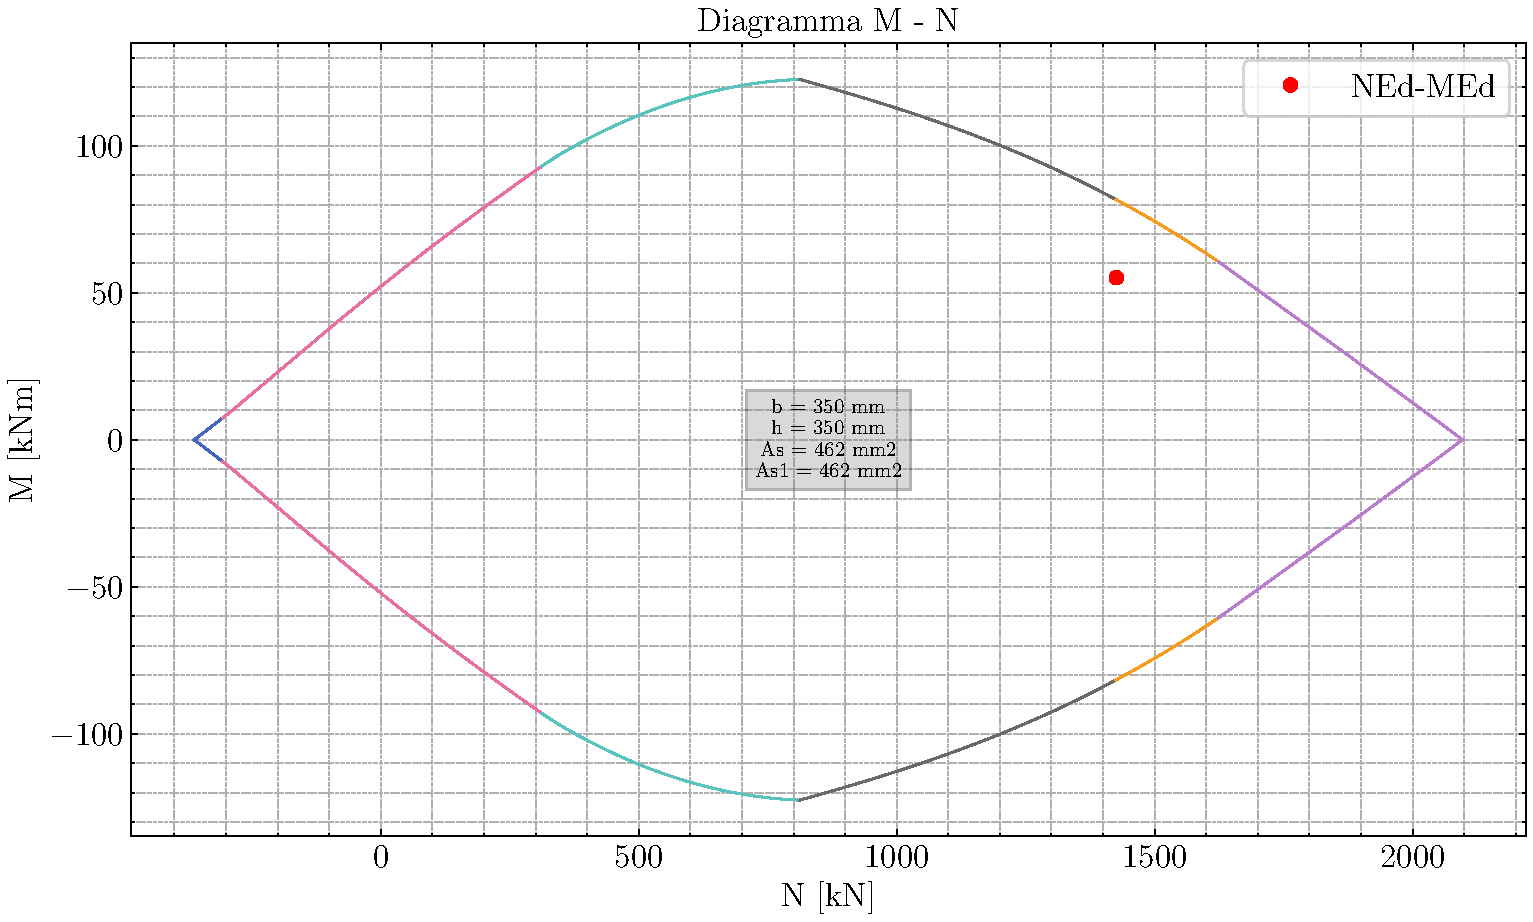
\includegraphics[width=\textwidth]{IMG/M_N_diagram_pilastro_secondo_ordine.pdf}
    \caption{Diagramma MN con sollecitazione flettente tenente conto degli effetti del secondo ordine tramite il metodo della curvatura nominale}
    \label{fig:MN_diagram_secondo_ordine}
\end{figure}